\documentclass{IEEEcsmag}

\usepackage[colorlinks,urlcolor=blue,linkcolor=blue,citecolor=blue]{hyperref}
\expandafter\def\expandafter\UrlBreaks\expandafter{\UrlBreaks\do\/\do\*\do\-\do\~\do\'\do\"\do\-}
\usepackage{upmath,color}

\usepackage[spanish]{babel}
%\usepackage[latin1]{inputenc}
\usepackage[utf8]{inputenc}  

\jvol{1}
\jnum{1}
\paper{1}
\jmonth{Noviembre}
\jname{ITICs letters}
\jtitle{Proyectos Integradores}
\pubyear{2023}
\usepackage{cite}
\usepackage{amsmath,amssymb,amsfonts}
\usepackage{algorithmic}
\usepackage{graphicx}
\usepackage{textcomp}
\usepackage{xcolor}
\usepackage{listings}

\newtheorem{theorem}{Theorem}
\newtheorem{lemma}{Lemma}


\setcounter{secnumdepth}{0}

\begin{document}

%imprimir código
\lstnewenvironment{javaCode}[1][]
{\lstset{
    language=Java,
    basicstyle=\scriptsize\ttfamily,
    numbers=none, % Modificado: quitar los números de línea
    keywordstyle=\color{blue},
    commentstyle=\color{gray},
    stringstyle=\color{purple},
    breaklines=true,
    breakatwhitespace=true,
    tabsize=4,
    showspaces=false,
    showstringspaces=false,
    frame=single,
    captionpos=b,
    floatplacement=!h,
    #1
}}
{}


\sptitle{Proyecto Integrador de Primer Semestre}

\title{Software de resolución de problemas de Ingeniería }

\author{Martinez Martinez Freyra Wendy}
\affil{Instituto Tecnológico Superior del Occidente del Estado de Hidalgo, Mixquiahuala, Hgo., 42700, Mexico}

\author{Mera Ibarra Carol}
\affil{Instituto Tecnológico Superior del Occidente del Estado de Hidalgo, Mixquiahuala, Hgo., 42700, Mexico}

\author{Gonzales Yañez Dulce Karen}
\affil{Instituto Tecnológico Superior del Occidente del Estado de Hidalgo, Mixquiahuala, Hgo., 42700, Mexico}

\author{Mendoza Calva Marco Antonio}
\affil{Instituto Tecnológico Superior del Occidente del Estado de Hidalgo, Mixquiahuala, Hgo., 42700, Mexico}

\author{Gómez Mejía Eduardo}
\affil{Instituto Tecnológico Superior del Occidente del Estado de Hidalgo, Mixquiahuala, Hgo., 42700, Mexico}

%\author{Third Author III}
%\affil{Institute, City, (State), Postal Code, Country}

\markboth{ITSOEH/ITICS/PROYECTO INTEGRADOR PRIMER SEMESTRE}{THEME/FEATURE/DEPARTMENT}

\begin{abstract}
Un resumen (abstract) es un párrafo único que resume los aspectos importantes del manuscrito. A menudo indica si el manuscrito es un informe de un trabajo nuevo, una revisión o una descripción general, o una combinación de ambos. No cite referencias en el resumen. Este tipo de documento debe incluir contenido propiedad de los autores; es decir, no debe contener contenido de otras fuentes, ademas la redacción debe  estar dirigida a un tipo de lector técnico general. Este archivo se encuentra disponible en \href{https://github.com/fcuadrosgithub/integrador-primero.git}{https://github.com/fcuadrosgithub/integrador-primero.git}.
\end{abstract}

\maketitle
\chapteri{D}urante este proyecto de software de resolución de problemas de ingeniería, trabajamos en equipo utilizando la metodología de las 6 D's para resolver ejercicios de geometría analítica, álgebra y matemáticas discretas con Java. Adquirimos experiencia en programación, además en desarrollo de soluciones prácticas mediante el cálculo de ecuaciones de rectas y ángulos, así como la resolución de ecuaciones cuadráticas y conversiones numéricas.

\clearpage

\section{Resolución Problema 1} 
Para dar solución a este problema se utiliza  el método de las 6’D, que está compuesto de seis etapas, cada una de las cuales consta de una serie de pasos, descripción del
problema, definición de solución, diseño de la solución,
desarrollo de la solución, depuración y pruebas y
documentación. \\



Este programa en Java resuelve dos problemas de geometría analítica. Primero, determina la ecuación de una recta que pasa por los puntos A y B usando el método:
\[
\text{ $y = mx + b$ }
\]
 Luego, calcula el ángulo interno entre la recta y el eje horizontal utilizando el método de la tangente inversa  $"a "$ = arctan(m)".
\subsection{\textbf{Descripcion del problema:}}
\begin{itemize}

    \item Dados 2 puntos A y B con coordenadas x1, y1 y x2, y2 respectivamente. Regresar la ecuación de la recta y el ángulo interno α que se forma entre el eje horizontal y la recta.
    \end{itemize}
\subsection{\textbf{Diseño de la solución:}}
La solución implica calcular la pendiente de la recta que pasa por los puntos A y B y utilizarla para obtener la ecuación de la recta en la forma y = mx + b, donde m es la pendiente y b es la intersección en el eje y. Una vez obtenida la ecuación de la recta, se puede calcular el ángulo interno utilizando la función trigonométrica arcotangente.
\begin{figure}[h!]
    \centering
    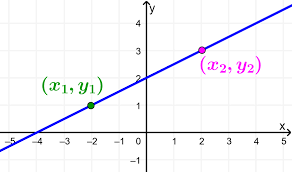
\includegraphics[width = 6.5 cm]{LaTeX/latex-imagenes/grafica-rectapendiente.png}
    \caption{Gráfica de dos puntos en la recta.}
    \label{fig:GraficaEcuacionRecta}
\end{figure} 
\subsection{\textbf{\textit{Diseño de solución }}}
\begin{itemize}
  \item Calcular la pendiente (m) de la recta utilizando la fórmula:
\begin{equation}
    m = (y2 - y1) / (x2 - x1)
\end{equation}
   
  \item  Calcular el término independiente (b)  utilizando la fórmula 
 \begin{equation}
     b = y1 - mx1.
\end{equation}
  \item Obtener la ecuación de la recta
   \begin{equation}
     y = mx + b.
\end{equation}
  \item Calcular el ángulo interno (a) utilizando la fórmula
    \begin{equation}
      a = tan^(-1)(m)
    \end{equation}
\end{itemize}
Utilizando este método, puedes encontrar la ecuación de la recta a partir de dos puntos. Recuerda que si los dos puntos son idénticos la recta será una linea vertical
\cite{rectaPendiente}

\subsection{ \textbf{\textit{Diagrama de flujo }}}

\begin{figure}[H]
    \centering
    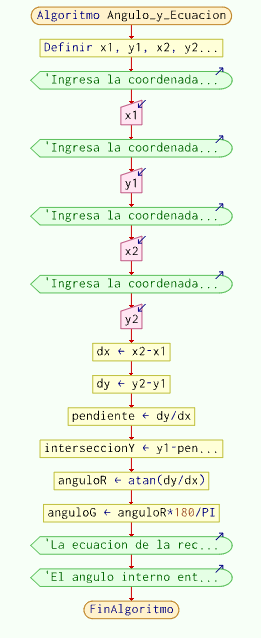
\includegraphics[width=6cm]{LaTeX/latex-imagenes/Diagrama de flujo.png}
    \caption{Diagrama de flujo usado para la solución del problema}
\end{figure}
\subsection{\textbf{Desarrollo de la solución:}}
// Comienza solicitando al usuario dos puntos $A(x_{1}, y_{1})$ y $B(x_{2}, y_{2})$.

\begin{lstlisting}[style=javaStyle]
    Scanner sc = new Scanner(System.in);
    // Solicita datos del primer punto
    System.out.println("Ingresa la coordenada x1: ");
    double x1 = sc.nextDouble();
    System.out.println("Ingresa la coordenada y1: ");
    double y1 = sc.nextDouble();
        
    // Solicita datos del segundo punto
    System.out.println("Ingresa la coordenada x2: ");
    double x2 = sc.nextDouble();
    System.out.println("Ingresa la coordenada y2: ");
    double y2 = sc.nextDouble();
\end{lstlisting}
//Se  calcula la diferencia entre coordenadas, con el fin de determinar la distancia o el desplazamiento entre dos puntos en un sistema de coordenadas.
\begin{lstlisting}[style=javaStyle]
    // Calcula la diferencia entre coordenadas
    double dx = x2 - x1;
    double dy = y2 - y1;
        
\end{lstlisting}
//Calculamos la pendiente usando la  formula 
 $m = (y2-y1) / (x2-x1)$
Una vez obtenida la pendiente, obtenemos la intersección con el eje "Y"
\begin{lstlisting}[style=javaStyle]
        // Calcula la pendiente y la intersección con el eje Y
        double pendiente = dy / dx;
        double interseccionY = y1 - pendiente * x1;
        
\end{lstlisting}
    // Calcula el ángulo en radianes
        
\begin{lstlisting}[style=javaStyle]
     double anguloR = Math.atan2(dy, dx);
\end{lstlisting}
    // Convierte el ánguloR a grados
\begin{lstlisting}[style=javaStyle]
    double anguloG = Math.toDegrees(anguloR);
\end{lstlisting}
    //Finalmente obtenemos como resultado la ecuación de la recta que pasa a través de dos puntos dados, A y B. 
    Además del el ángulo interno formado entre el eje horizontal y la recta.
\begin{lstlisting}[style=javaStyle]
    
        // Imprime la ecuación y el ángulo interno
        System.out.println("La ecuación de la recta es: y = " + pendiente + "x + " + interseccionY);
        System.out.println("El ángulo interno entre la recta y el eje horizontal es: " + anguloG + " grados");

\end{lstlisting}

\subsection{\textbf{\textit{Código general}}}
\begin{lstlisting}[style=javaStyle]
package com.mycompany.proyecto;
import java.util.Scanner;
/**
 *
 * @author Frey
 */
public class Angulo_y_Ecuacion {
    public static void main(String[] args) {
        Scanner sc = new Scanner(System.in);
        // Solicita datos del primer punto
        System.out.println("Ingresa la coordenada x1: ");
        double x1 = sc.nextDouble();
        System.out.println("Ingresa la coordenada y1: ");
        double y1 = sc.nextDouble();
        
        // Solicita datos del segundo punto
        System.out.println("Ingresa la coordenada x2: ");
        double x2 = sc.nextDouble();
        System.out.println("Ingresa la coordenada y2: ");
        double y2 = sc.nextDouble();
        
        // Calcula la diferencia entre coordenadas
        double dx = x2 - x1;
        double dy = y2 - y1;
        
        // Calcula la pendiente y la intersección con el eje y
        double pendiente = dy / dx;
        double interseccionY = y1 - pendiente * x1;
        
        // Calcula el ángulo en radianes
        double anguloR = Math.atan2(dy, dx);
        
        // Convierte el ánguloR a grados
        double anguloG = Math.toDegrees(anguloR);
        
        // Imprime la ecuación y el ángulo interno
        System.out.println("La ecuación de la recta es: y = " + pendiente + "x + " + interseccionY);
        System.out.println("El ángulo interno entre la recta y el eje horizontal es: " + anguloG + " grados");
    }
}
\end{lstlisting}


\subsection{\textbf{Depuración y pruebas:}}
\begin{figure}[H]
    \centering
    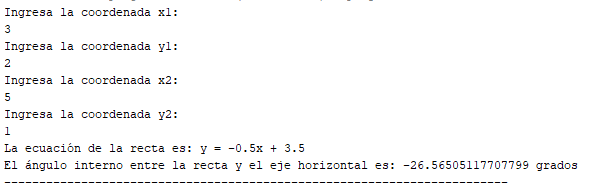
\includegraphics[width=8cm]{LaTeX/latex-imagenes/prueba de escritorio2.png}
    \caption{Prueba de escritorio.}
\end{figure}
\begin{figure}[H]
    \centering
    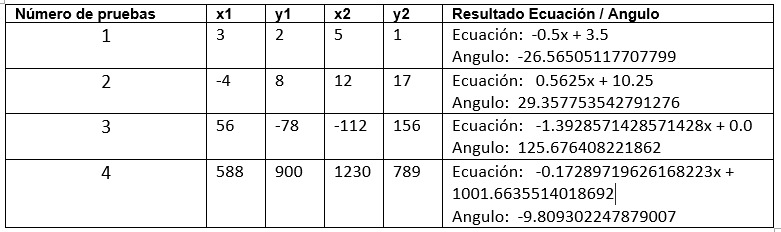
\includegraphics[width=10cm]{LaTeX/latex-imagenes/TABLA.jpg}
    \caption{Tabla de corridas.}
\end{figure}

\clearpage

\section{Resolución Problema 2} 
En el siguiente informe se emplea la metodología de las 6 D´s, el cual tiene como objetivo presentar el desarrollo y los resultados obtenidos de la elaboración de un programa en Java que permite resolver ecuaciones cuadráticas utilizando la fórmula general, dando lugar a tres posibles resultados.
\subsection{\textbf{Descripción del problema:}}
Dada una ecuación cuadrática regresar los valores de las raíces en caso de que estén sobre el conjunto de los números reales, en caso contrario indicar que la solución está en el conjunto de los números complejos. El principal objetivo será encontrar el valor de “x” para lograr que la ecuación sea verdadera.
\subsection{\textbf{Definición de solución:}}
La forma general de la ecuación de segundo grado es la siguiente:

\begin{equation}
    ax^{2}+bx+c=0  
    \label{eqn:ecuacioncuadratica}
\end{equation}
A continuación se muestra la fórmula general, con la cual se realiza la sustitución de los valores correspondientes a “a”, “b” y “c” de acuerdo a la ecuación de segundo grado (1) que se desee resolver y por ende, conocer su resultado.

\begin{equation}
    \frac{-b\pm\sqrt{b^2-4ac}}{2a}
\end{equation}

Es importante saber que el resultado puede variar en ninguna, una o dos soluciones reales.

La representación gráfica es la siguiente:

\begin{figure}[!ht]
\centering
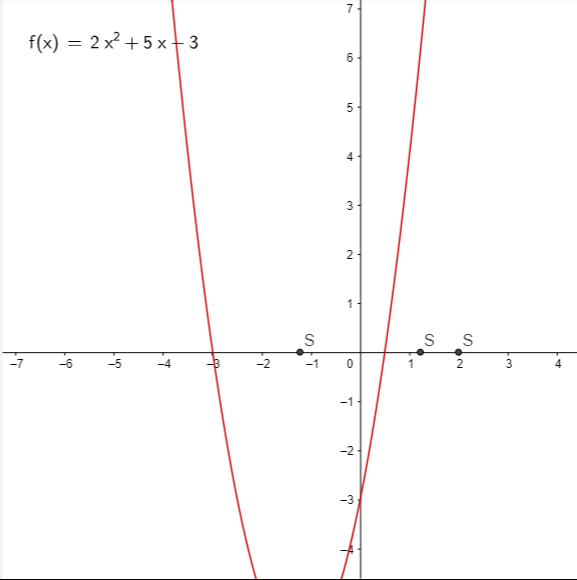
\includegraphics[width=6cm]{LaTeX/latex-imagenes/ejemploGrafica.png}
\caption{Gráfica de una ecuación cuadrática con dos soluciones.}
\label{fig:grafica}
\end{figure}

\newline
\subsection{\textbf{Diseño de la solución:}}
Para lleva a cabo la elaboración del código de java, se requiere diseñar el proceso para asegurar que el progreso sea correcto.

%diagrama
\begin{figure}[H]
\centering
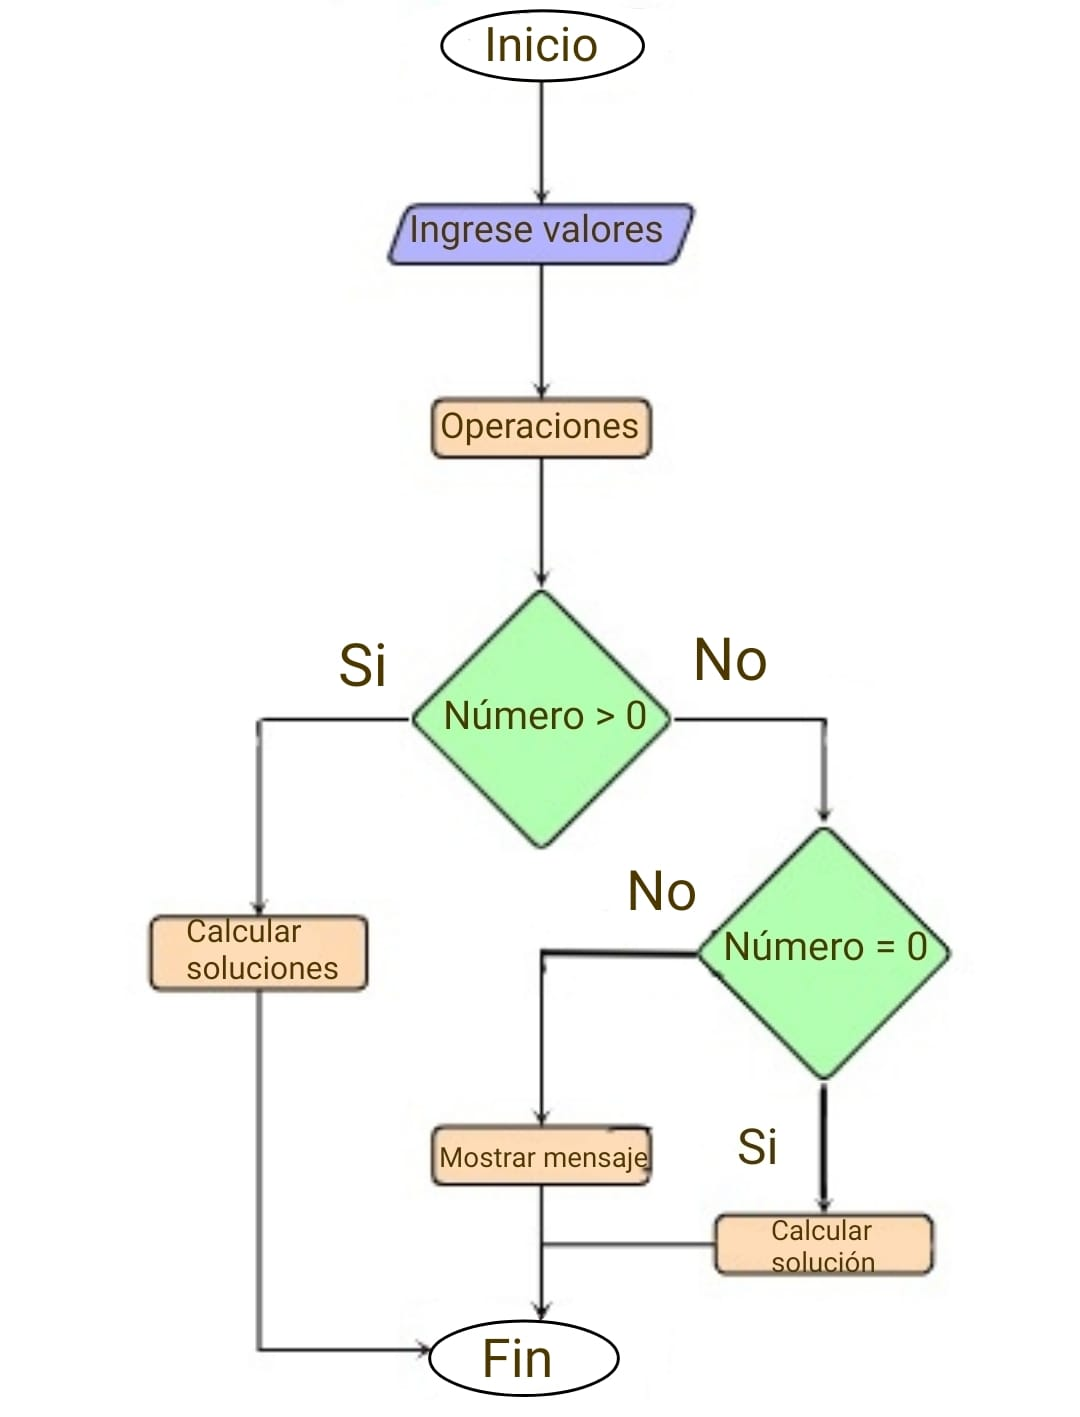
\includegraphics[width=6cm]{LaTeX/latex-imagenes/diagramaflujo.jpg}
\caption{Diagrama de flujo que muestra el proceso para resolver la fórmula general.}
\label{fig:diagrama_flujo}
\end{figure}

\newline

Prosiguiendo con el diseño, ahora se va a mostrar el código como resultado de la elaboración del diagrama donde:

\begin{itemize}
  \item El usuario debe ingresar tres valores, es decir, los coeficientes pertenecientes a la forma estándar de la ecuación cuadrática.
  \item El programa realiza las operaciones correspondientes a la fórmula general.
  \item Al final el o los resultado serán mostrados.
\end{itemize}
\subsection{\textbf{Desarrollo de la solución:}}
\subsection{Programa en Java}
En seguida, se muestra el código del programa.
Se utiliza la clase Scanner y la clase Random que se encuentran en el paque de java.util, y además se agrega el tipo de dato.

\begin{lstlisting}[style=javaStyle]
public static void main(String[] args) {
        Scanner constante = new Scanner(System.in);

        double a, b, c, numero, x1, x2, x;
\end{lstlisting}
**
%codigo
El usuario ingresa los valores solicitados, siendo las variables ``a", ``b'' y ``c". Posteriormente se cierra el escaneo.

\begin{lstlisting}[style=javaStyle]
//Solicita el valor de los coeficientes para realizar la ecuación
        System.out.print("Ingrese el valor de a: ");
        a = constante.nextDouble();
        
        System.out.print("Ingrese el valor de b: ");
        b = constante.nextDouble();
        
        System.out.print("Ingrese el valor de c: ");
        c = constante.nextDouble();
        //Cierra el escaneo
        constante.close();

\end{lstlisting}

Continúa cerrando  y a realizar las primeras operaciones de la fórmula general, que serán determinantes para la siguiente condición de la estructura de control if.

\begin{lstlisting}[style=javaStyle]
        //Cierra el escaneo
        constante.close();
        
        numero = b * b - 4 * a * c;
\end{lstlisting}
Prosiguiendo con la operación de la fórmula general, ahora se debe determinar cuál será la respuesta dependiendo del resultado de la operación anterior, entonces la estructura de control if va a permitir tomar decisiones en función de la condición y así llegar a un resultado.

\begin{lstlisting}[style=javaStyle]
   //Se va a determinar cuál de las tres posibles soluciones es 
       // la indicada dependiendo de los valores ingresados
        if (numero > 0) {
            x1 = (-b + Math.sqrt(numero)) / (2 * a);
            x2 = (-b - Math.sqrt(numero)) / (2 * a);
            System.out.println("Tiene dos soluciones, las cuales son x1 = " + x1 + " y x2 = " + x2);
        } else if (numero == 0) {
            x = -b / (2 * a);
            System.out.println("Solo tiene una solución, la cual es x = " + x);
        } else {
            System.out.println("La ecuación no tiene soluciones reales.");
        }
\end{lstlisting}
 Después de que la condición evaluada sea verdadera, procede a imprimir en la consola el resultado de las operaciones de la fórmula general realizadas junto con el mensaje correspondiente.

\subsection{Código completo}
\begin{lstlisting}[style=javaStyle]
import java.util.Scanner;

public class ecuacionCuadratica {

    public static void main(String[] args) {
        Scanner constante = new Scanner (System.in); 
        
       double a, b, c, numero, x1, x2, x;
        //Solicita el valor de los coeficientes para realizar la ecuación
        System.out.print("Ingrese el valor de a: ");
        a = constante.nextDouble();
        
        System.out.print("Ingrese el valor de b: ");
        b = constante.nextDouble();
        
        System.out.print("Ingrese el valor de c: ");
        c = constante.nextDouble();
        //Cierra el escaneo
        constante.close();
        
        numero = b * b - 4 *a * c;
        //Se va a determinar cuál de las tres posibles soluciones es la indicada dependiendo de los valores ingresados
        if (numero > 0){
            x1 = (-b + Math.sqrt(numero)) / (2* a);
            x2 = (-b - Math.sqrt(numero)) / (2* a);
            System.out.println("Tiene dos soluciones, las cuales son x1 = " + x1 + " y x2 = " + x2);
            
        } else if (numero == 0){
            x = -b / (2*a);
            System.out.println("Solo tiene una solución, la cual es es x = " + x);
        }else {
            System.out.println("La ecuación no tiene soluciones reales.");
        }
    }
}



\end{lstlisting}
\subsection{\textbf{Depuración y pruebas:}}
Comprobación del funcionamiento a través de pruebas, ingresando los valores solicitados al usuario y ejecutando en Java, un total de cinco veces.
\begin{figure}[!ht]
\centering
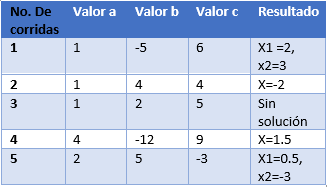
\includegraphics[width=6cm]{LaTeX/latex-imagenes/tablaprueba.png}
\caption{Prueba de escritorio.}
\label{fig:diagrama_flujo}
\end{figure}
\clearpage

\section{Resolución Problema 3}
La busqueda de la distancia entre dos puntos y la verificación de si se encuentran dentro de una circunferencia en Java es posible crear un programa que realice estos cálculos y determine la ubicación de los puntos con respecto a una circunferencia proporcionada por el usuario.
Para calcular la distancia entre dos puntos, se utiliza la fórmula de la distancia. Esta fórmula nos permite obtener una medida precisa de la distancia en un plano, teniendo en cuenta las coordenadas x,y de los puntos.
El programa calculará la distancia entre los puntos utilizando la fórmula mencionada y luego utilizará una estructura condicional para determinar si los puntos se encuentran dentro de la circunferencia o fuera de ella, en función del radio ingresado.
De esta manera, el programa en Java proporcionará una solución eficiente y precisa para determinar la ubicación de los puntos en relación con la circunferencia, basándose en el cálculo de la distancia y el uso de una estructura condicional.
\subsection{\textbf{Descripción del problema:}}
\begin{enumerate}
    \item el problema tiene como objetivo determinar si un punto $T$ con coordenadas $(x_{2}, y_{2})$ se encuentra dentro del área de una circunferencia. El usuario proporcionará las coordenadas $(x_{1}, y_{1})$ del centro de la circunferencia, las coordenadas $(x_{2}, y_{2})$ del punto $T$, y el radio $r$. El proceso implica utilizar la ecuación de distancia entre dos puntos y presentar la respuesta resultante.
\end{enumerate}
\begin{figure}[h!]
    \centering
    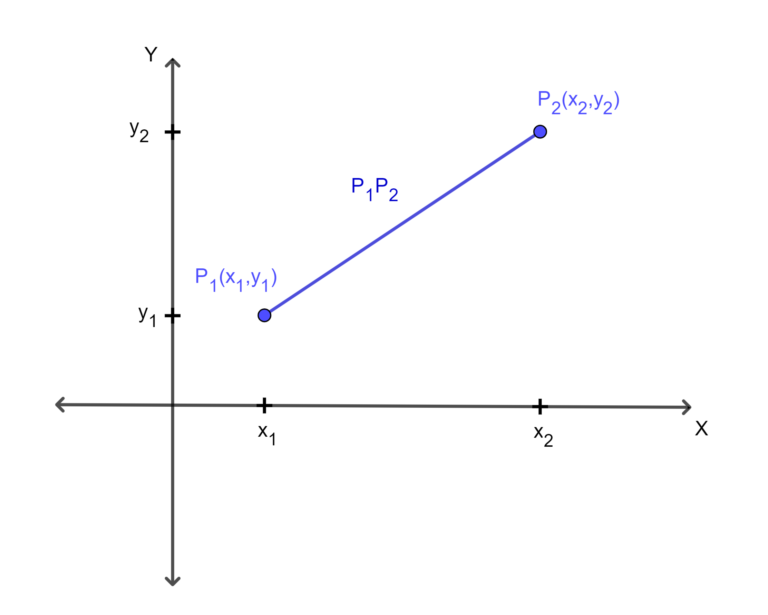
\includegraphics[width=1\linewidth]{LaTeX//latex-imagenes/Distancia_entre_dos_puntos-2-768x615.png}
    \caption{La distancia entre dos puntos.}
    \label{fig:enter-label}
\end{figure}
\subsection{\textbf{Definición de solución:}}
La solución consiste en evaluar si un punto $T$ con coordenadas $(x_{2}, y_{2})$ está dentro del área de una circunferencia con centro en $(x_{1}, y_{1})$ y radio $r$. Para ello se utiliza la fórmula de la distancia entre dos puntos y se compara la distancia calculada con el radio $r$ de la circunferencia:
    \begin{equation}
        \text{distancia} = \sqrt{ (x_2 - x_1)^2 + (y_2 - y_1)^2 }
    \end{equation}
    
    \begin{enumerate}
        \item Si la distancia es mayor que el radio $r$, el punto $T$ está fuera de la circunferencia.
        \item Si la distancia es igual al radio $r$, el punto $T$ está en el borde de la circunferencia.
        \item Si la distancia es menor que el radio $r$, el punto $T$ está dentro del área de la circunferencia.
    \end{enumerate}
\subsection{\textbf{Diseño de la solución:}}
\begin{enumerate} 
    \item Solicitar al usuario las coordenadas del centro de la circunferencia $(x_{1}, y_{1})$, las coordenadas del punto $T$ $(x_{2}, y_{2})$, y el radio $r$.
    
    \item Calcular la distancia entre el centro y el punto $T$ utilizando la fórmula de distancia entre dos puntos:
    \begin{equation}
        \text{distancia} = \sqrt{ (x_2 - x_1)^2 + (y_2 - y_1)^2 }
    \end{equation}

    \item Verificar si la distancia calculada es mayor que el radio $r$:
    \begin{enumerate}
        \item Si es mayor, el punto $T$ está fuera de la circunferencia.
    \end{enumerate}
    
    \item Verificar si la distancia calculada es igual al radio $r$:
    \begin{enumerate}
        \item Si es igual, el punto $T$ está en el borde de la circunferencia.
    \end{enumerate}

    \item Verificar si la distancia calculada es menor que el radio $r$:
    \begin{enumerate}
        \item Si es menor, el punto $T$ está dentro del área de la circunferencia.
    \end{enumerate}
    
    \item Presentar el resultado al usuario.
    
\end{enumerate}

\begin{figure}[h!]
    \centering
    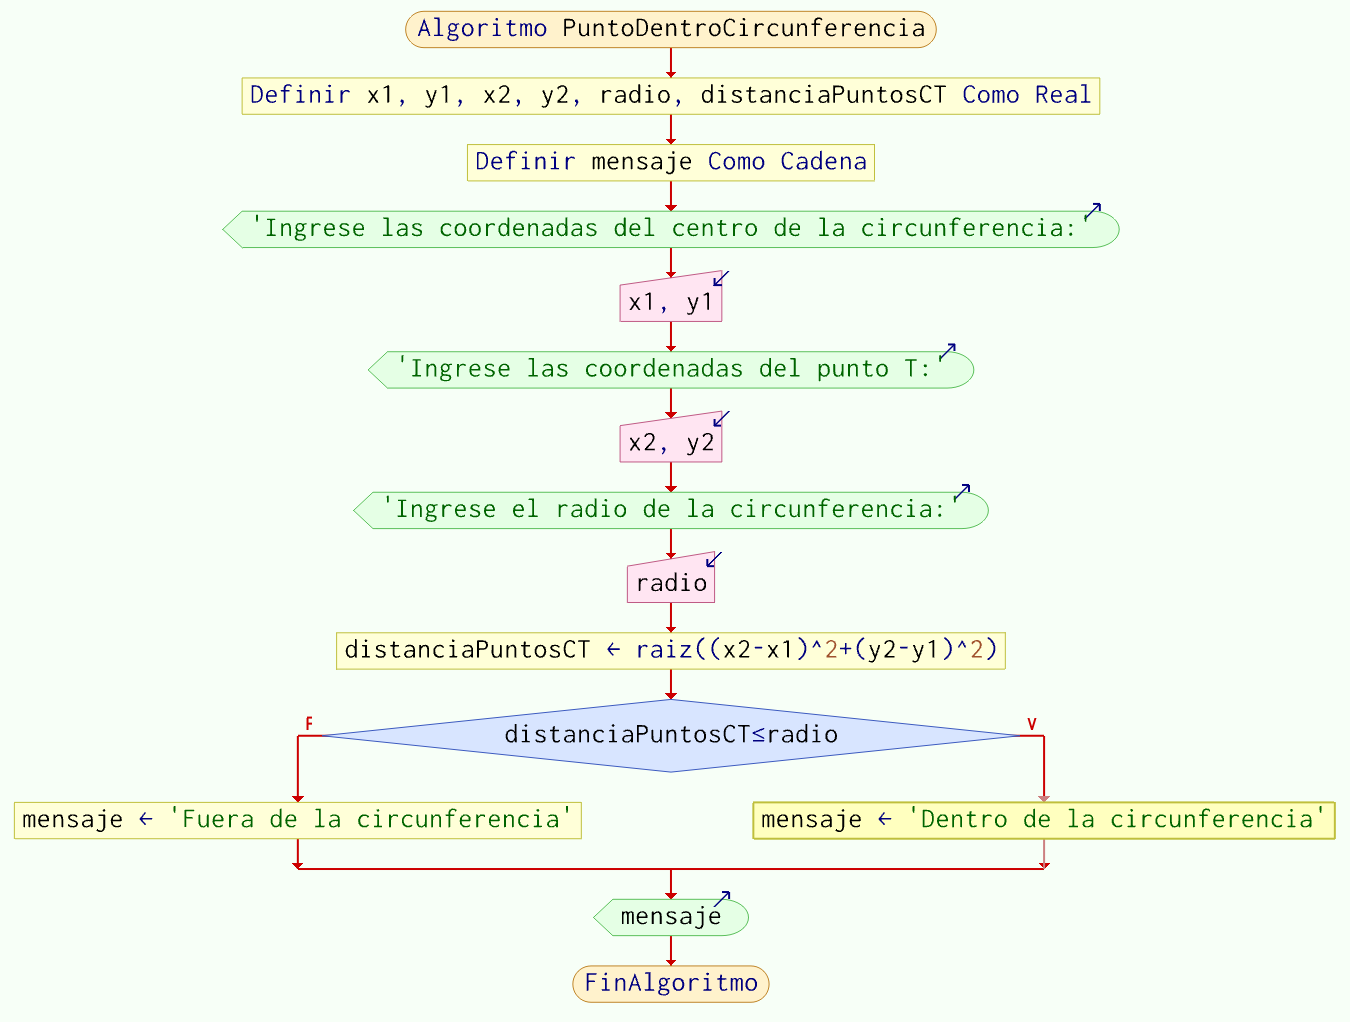
\includegraphics[width=1\linewidth]{LaTeX//latex-imagenes/Captura de pantalla 2023-11-23 150737.png}
    \caption{Diagrama de flujo.}
    \label{fig:enter-label}
\end{figure}
\subsection{\textbf{Desarrollo de la solución:}}
Programa en Java.
\newline
    
Se utiliza un objeto Scanner para obtener datos de entrada desde la consola.\\ Se solicitan al usuario las coordenadas del centro de una circunferencia (punto C), el radio de la circunferencia y las coordenadas de un punto T. \\
    Los valores ingresados se almacenan en arreglos de cadenas de caracteres y se cierra el objeto Scanner para liberar recursos.
\newline
    \begin{javaCode}
        Scanner datos = new Scanner(System.in);
        System.out.println("Ingresa las coordenadas del centro de una circunferencia (punto C) separado por una coma (x,y):");
        String[] puntoC = (datos.nextLine()).split(",");
        System.out.println("Ingresa el radio de la circunferencia:");
        float radio = datos.nextFloat();
        datos.nextLine();
        System.out.println("Ingresa los valores de \"x\" y \"y\" del punto a evaluar (punto T) separado por una coma (x,y):");
        String[] puntoT = (datos.nextLine()).split(",");
        datos.close();
    \end{javaCode} 
    % Bloque de Procedimientos
Se convierten las coordenadas del punto C y del punto T de cadenas de caracteres a números enteros (int). \\
    Luego, se utiliza la fórmula de la distancia para calcular la distancia entre los puntos C y T, almacenando el resultado como un número de punto flotante (float).
    
    \begin{javaCode}
        int xc = Integer.parseInt(puntoC[0].trim());
        int yc = Integer.parseInt(puntoC[1].trim());
        int xt = Integer.parseInt(puntoT[0].trim());
        int yt = Integer.parseInt(puntoT[1].trim());
        float distanciaPuntosCT = (float)Math.sqrt(Math.pow(xt-xc, 2) + Math.pow(yt-yc, 2));
    \end{javaCode}
    
    % Bloque de Salida de Datos
    Se declara una cadena de caracteres vacía llamada "mensaje". \\
    Se utiliza una estructura condicional para determinar la posición relativa del punto T con respecto a la circunferencia y asignar un mensaje correspondiente. Finalmente, se imprime el mensaje en la consola.
    
    \begin{javaCode}
        String mensaje = "";
        if (distanciaPuntosCT > radio) {
            mensaje = "El punto T("+xt+","+yt+") esta fuera de la circunferencia";
        } else if (distanciaPuntosCT == radio) {
            mensaje = "El punto T("+xt+","+yt+") esta en la circunferencia";
        } else {
            mensaje = "El punto T("+xt+","+yt+") esta dentro de la circunferencia";
        }
        System.out.println(mensaje);
    \end{javaCode}
\subsection{\textbf{Depuración y pruebas:}}
\begin{figure}[h!]
    \centering
    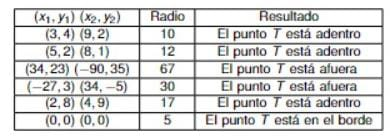
\includegraphics[width=1\linewidth]{c8e8865c-0fa3-4437-b97a-0e67eb053d1f.jpg}
    \caption{Tabla de pruebas}
    \label{fig:enter-label}
\end{figure}
\clearpage

\section{Resolución Problema 4}

\subsection{\textbf{INTRODUCCIÓN} } 

El sistema binario es un sistema numérico que se compone únicamente de dos dígitos, 0 y 1, utilizados para representar valores. La conversión de números decimales (base 10) a números binarios (base 2) . El propósito de este proyecto es desarrollar un algoritmo eficiente para convertir números decimales enteros, tanto positivos como negativos, a su equivalente binario.

La metodología para convertir un número decimal entero a binario implica dividir de forma sucesiva el número decimal entre 2 y registrar el residuo de cada división. Estos residuos son  leídos de abajo hacia arriba y conformarán el número binario equivalente. En el caso de números negativos, se utiliza el complemento a dos para representar tanto el signo como el valor absoluto del número.


El resultado del  algoritmo desarrollado se va a demostrar ser  preciso y eficiente en la conversión de números decimales enteros a binarios. A través de pruebas y verificaciones, el algoritmo proporcionara resultados correctos y coherentes para distintos valores de entrada. Esto permitirá una conversión confiable y precisa de números decimales enteros a binarios, lo cual resultara fundamental en diversas aplicaciones.


\subsection{\textbf{Descripción del problema:}}

\subsection{\textbf{DESCRIPCIÓN DEL PROBLEMA} } 
Implica comprender y definir claramente el problema que se quiere resolver. En este caso, se trata de convertir un número decimal a binario.


\begin{figure}[h!]
    \centering
    \includegraphics[width = 6 cm]{LaTeX/latex-imagenes/DECIMAL.png}
    \caption{Decimal a binario}
    \label{decimal a binario}
\end{figure}


\subsection{\textbf{Definición de solución:}}

\subsection{\textbf{DEFINICIÓN DE SOLUCIÓN} }
En esta etapa, se determina el enfoque o algoritmo general que se utilizará para convertir el número decimal a binario. 


%diagrama
\begin{figure}[H]
\centering
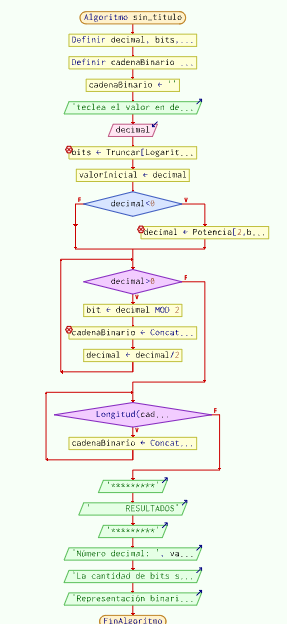
\includegraphics[width=6cm]{LaTeX/latex-imagenes/1.png}
\caption{Diagrama de flujo que muestra el proceso para resolver }
\label{fig:diagrama_flujo}

\end{figure}


\subsection{\textbf{Diseño de la solución:}}

\subsection{\textbf{DISEÑO DE SOLUCIÓN} }
\subsection{\textbf{\textit{Programa en Java}}}
Se detallan los pasos específicos y la lógica necesaria para implementar el algoritmo definido anteriormente. Se pueden utilizar diagramas, pseudocódigo u otras herramientas para representar visualmente el flujo de la solución.

\subsectionse \textit{\textbf{solicita al usuario que teclee el valor decimal}}

\begin{lstlisting}[style=javaStyle]
package com.mycompany.programacorrecto;

import java.util.Scanner;

/**MARCO ANTONIO MENDOZA CALVA
 */
 public class Programacorrecto {

    public static void main(String[] args) {
     Scanner h=new Scanner(System.in);
     System.out.println("Teclea el valor en decimal : ");
\end{lstlisting}
**
%codigo
\subsectionse\textbf{\textit{calcula los bits del numero entero que dio el usuario}}

\begin{lstlisting}[style=javaStyle]
int decimal=h.nextInt();
     int bits = (int) (Math.log(Math.abs(decimal)) / 
     Math.log(2)) + 1;//calcular los bits del numero entero.
\end{lstlisting}

\subsectionse\textbf{\textit{Verificar si el número es negativo (-)}}

\begin{lstlisting}[style=javaStyle]
        int valorinicial=decimal;    
    
       
        // Verificar si el número es negativo (-)
        if (decimal < 0) {
\end{lstlisting}

\subsectionse\textbf{\textit{Obtener la representación en complemento a 2}}

\begin{lstlisting}[style=javaStyle]
  // Obtener la representación en complemento a 2
            decimal = (int) (Math.pow(2, bits) + decimal);
        }
\end{lstlisting}
\subsectionse\textbf{\textit{Convertir Numero decimal a binario}}

\begin{lstlisting}[style=javaStyle]
  // Convertir Numero decimal a binario
        StringBuilder binary = new StringBuilder();
        do {
\end{lstlisting}


\subsectionse\textbf{\textit{Obtener el bit menos significativo}}

\begin{lstlisting}[style=javaStyle]
  // Obtener el bit menos significativo
            int bit = decimal % 2;
\end{lstlisting}
\subsectionse\textbf{\textit{Agregar el bit al inicio de la cadena}}

\begin{lstlisting}[style=javaStyle]
  // Agregar el bit al inicio de la cadena
            binary.insert(0, bit);

\end{lstlisting}

\subsectionse\textbf{\textit{Dividir el número por 2}}

\begin{lstlisting}[style=javaStyle]
   // Dividir el número por 2
            decimal /= 2;
        } while (decimal > 0);

\end{lstlisting}

\subsectionse\textbf{\textit{Ajustar la longitud al número de bits especificado}}

\begin{lstlisting}[style=javaStyle]
    // Ajustar la longitud al número de bits especificado
        while (binary.length() < bits) {
            binary.insert(0, '0');
        }

\end{lstlisting}

\subsectionse\textbf{\textit{converitr a cadena}}

\begin{lstlisting}[style=javaStyle]
    String binario =binary.toString(); //

\end{lstlisting}
\subsectionse\textbf{\textit{final mente se obtienen los resultados}}

\begin{lstlisting}[style=javaStyle]
     System.out. println("       RESULTADOS    ");
        System.out.println("El Número decimal es : \t" + valorinicial);
        System.out. println("La cantidad de bits son: \t "+ bits);
        System.out.println("El numero binario es :\t " + binario);
    }       
}

\end{lstlisting}


\subsection{\textbf{Desarrollo de la solución:}}

\subsection{\textbf{DESARROLLO DE SOLUCIÓN }}
Implementa el algoritmo utilizando un lenguaje de programación específico. Se escriben líneas de código que siguen la lógica y los pasos definidos en la etapa de diseño. Es importante asegurarse de que el código sea claro, legible y esté correctamente estructurado.
\subsection{\textbf{Código completo}}
\begin{lstlisting}[style=javaStyle]
package com.mycompany.programacorrecto;

import java.util.Scanner;

/**MENDOZA CALVA MARCO ANTONIO

 */
public class Programacorrecto {

    public static void main(String[] args) {
     Scanner h=new Scanner(System.in);
     System.out.println("Teclea el valor en decimal : ");
     int decimal=h.nextInt();
     int bits = (int) (Math.log(Math.abs(decimal)) / Math.log(2)) + 1;//calcular los bits del numero entero.
     int valorinicial=decimal;    
    
       
        // Verificar si el número es negativo (-)
        if (decimal < 0) {
            // Obtener la representación en complemento a 2
            decimal = (int) (Math.pow(2, bits) + decimal);
        }

        // Convertir Numero decimal a binario
        StringBuilder binary = new StringBuilder();
        do {
            // Obtener el bit menos significativo
            int bit = decimal % 2;
            // Agregar el bit al inicio de la cadena
            binary.insert(0, bit);
            // Dividir el número por 2
            decimal /= 2;
        } while (decimal > 0);

        // Ajustar la longitud al número de bits especificado
        while (binary.length() < bits) {
            binary.insert(0, '0');
        }

        
        String binario =binary.toString(); //converitr a cadena 
        System.out. println("       RESULTADOS    ");
        System.out.println("El Número decimal es : \t" + valorinicial);
        System.out. println("La cantidad de bits son: \t "+ bits);
        System.out.println("El numero binario es :\t " + binario);
    }       
}

\end{lstlisting}


\subsection{\textbf{Depuración y pruebas:}}

\subsection{\textbf{DEPURACIÓN Y PRUEBAS} }
 verifica y corrige cualquier error que pueda existir en el código. Se realizan pruebas exhaustivas utilizando diferentes casos de prueba, incluyendo números decimales enteros positivos y negativos, para garantizar que la conversión a binario funcione correctamente en todos los escenarios posibles.

 \begin{figure}[h!]
    \centering
    \includegraphics[width = 6 cm]{LaTeX/latex-imagenes/PRUEBA.png}
    \caption{ CORRIDA}
    \label{codigo de java }
\end{figure}

\begin{figure}[h!]
    \centering
    \includegraphics[width = 6 cm]{LaTeX/latex-imagenes/tabla.png}
    \caption{ TABLA DE CORRIDAS }
    \label{codigo de java }
\end{figure}
\vspace*{-8pt}
\clearpage

\section{Resolución Problema 5}
Dado un numero binario de $n$ bits regresa su equivalente a decimal.


\subsection{\textbf{Descripción del problema:}}

La conversión de binario a decimal se logra multiplicando cada bit por su potencia de 2 correspondiente y sumando estos productos. La fórmula fundamental es la suma ponderada de los bits.


Se requiere convertir números binarios a su equivalente decimal.

\subsection{\textbf{Definición de solución:}}
La solución para convertir un número binario de n bits a su equivalente en decimal consiste en recorrer cada bit del número binario, multiplicar su valor por 2 elevado a la potencia correspondiente según su posición, y sumar los resultados. Al finalizar el recorrido, el valor obtenido será el equivalente decimal del número binario. Es importante verificar la validez del número binario y asegurarse de que esté compuesto únicamente por 0 y 1. El resultado se muestra como el equivalente decimal del número binario.


\subsection{\textbf{Diseño de la solución:}}
El programa solicita al usuario que ingrese un número binario de n bits. Se asegura de que el número ingresado consista únicamente en dígitos binarios 0 y 1. Si se detecta algún dígito decimal, el programa no funcionará.

Luego, se realiza la conversión del número binario ingresado a su equivalente decimal utilizando la fórmula de posición y peso explicada anteriormente.

Finalmente, el programa imprime el resultado de la conversión, es decir, el número decimal equivalente al número binario ingresado por el usuario.

\subsection{\textbf{Diseño de solución}}

\begin{figure}[H]
    \centering
    \includegraphics[width=6cm]{LaTeX/IMA/EL MERO MERO.png}
    \caption{Diagrama de flujo usado como base .}
\end{figure}


\subsection{\textbf{Desarrollo de la solución:}}
El desarrollo del código del programa en Java para la conversión de números binarios a decimales:

\begin{lstlisting}[style=javaStyle]
import java.util.Scanner;
import java.math.BigInteger;

public class NewClass {
    public static void main(String[] args) {
        Scanner bin = new Scanner(System.in);
        boolean continuar = true;
\end{lstlisting}
En esta paso en el programa son colocadas las variables $Scanner$ $BigInteger$
las cuales ayudaran al correr el programa

Se solicita al usuario ingresar un numero binario
\begin{lstlisting}[style=javaStyle]
// Bucle que permite al usuario ingresar números binarios hasta que ingrese 'x'

        while (continuar) {
        
            System.out.print("Ingrese un número en binario (o 'x' para terminar ): ")
            
            String entrada = bin.nextLine();
\end{lstlisting}

 La variable $while$ es utilizada como un "mientras" esta mantiene un bucle regresando a pedirnos un numero binario para su conversión a binario

\begin{lstlisting}[style=javaStyle]
                 // Si se ingresa 'x', el bucle se detiene;
            if (entrada.equalsIgnoreCase("x")) {
                continuar = false;
                continue;
            }
\end{lstlisting}

En esta línea, se declara una variable llamada decimal del tipo BigInteger. Se utiliza para almacenar el valor decimal resultante después de convertir el número binario ingresado. La función convertirBinarioADecimal se llama con el argumento entrada, que es el número binario ingresado por el usuario.

\begin{lstlisting}[style=javaStyle]
 // llama al método convertirBinarioADecimal para convertir el número binario ingresado a decimal
 
            BigInteger decimal = convertirBinarioADecimal(entrada);
            
\end{lstlisting}

 Esta línea imprime en la consola el mensaje "El número en decimal es: " seguido del valor almacenado en la variable decimal. Es decir, muestra el resultado de la conversión en formato decimal.

\begin{lstlisting}[style=javaStyle]
System.out.println("El número en decimal es: " + decimal);

\end{lstlisting}

Estas líneas definen el método convertirBinarioADecimal, que toma un argumento de tipo String llamado binario. El método crea un nuevo objeto BigInteger utilizando el constructor que toma dos argumentos: el número binario (binario) y la base (2) que se utiliza para interpretar el número binario y convertirlo a decimal. 

\begin{lstlisting}[style=javaStyle]
lic static BigInteger convertirBinarioADecimal(String binario) {
        return new BigInteger(binario, 2);

\end{lstlisting}

\text La fórmula se basa en el hecho de que cada posición en un número binario representa una potencia de 2. El dígito en la posición más a la derecha tiene un peso de \(2^0\), el siguiente dígito tiene un peso de \(2^1\), el siguiente tiene un peso de \(2^2\), y así sucesivamente.
\space

\begin{equation}

M = D0 * 2^0 + D1 * 2^1 + D2 * 2^2

\end{equation}


\subsection{\textbf{Depuración y pruebas:}}
En esta tabla se dasarrollan una seria de pruebas, 
\begin{figure}[H]
    \centering
    \includegraphics[width=10cm]{IMA/TABLA LA REAL.png}
    \caption{Prueba de escritorio.}
\end{figure}

\clearpage

\section{Resolución Problema 6}

\subsection{\textbf{Descripción del problema:}}

\subsection{\textbf{Definición de solución:}}

\subsection{\textbf{Diseño de la solución:}}

\subsection{\textbf{Desarrollo de la solución:}}

\subsection{\textbf{Depuración y pruebas:}}
\clearpage


\section{CONCLUSION}
En conclusión , los programas presentados demuestran un rendimiento satisfactorio en sus funciones fundamentales. Sin embargo, existe margen para mejorarlos al incorporar información adicional pertinente a cada problema específico. Esta mejora sería beneficiosa para lograr una mayor precisión y comprensión de los resultados obtenidos, permitiendo así adaptar los programas de acuerdo a las necesidades individuales de los usuarios.
\vspace*{-8pt}


\section{AGRADECIMIENTOS}
Esta sección es opcional. Si los autores creen necesario agradecer a alguien por haber aportado al desarrollo de su proyecto integrador de alguna u otra forma, esta sección esta destinada para esto.


\def\refname{REFERENCES}

\begin{thebibliography}{1}

\bibitem{AA1}
G. M. Amdahl, G. A. Blaauw, and F. P. Brooks, ``Architecture of the IBM System/360,'' {\it IBM J. Res. Dev}., vol. 8, no. 2, pp. 87--101, 1964. (Journal)

\bibitem{BB1}
IBM Corporation, IBM Knowledge Center - IBM Secure Service Container (Secure Service Container). [Online]. Available: {https://www.ibm.com/support/\break knowledgecenter/en/HW11R/com.ibm.hwmca.kc\_se.doc/\break introductiontotheconsole/wn2131zaci.html} (URL)

\bibitem{CC1}
J. Williams, ``Narrow-band analyzer,'' Ph.D. dissertation, Dept.  Elect. Eng., Harvard Univ., Cambridge, MA, USA, 1993. (Thesis or dissertation)

\bibitem{DD1}
J. M. P\'erez, R. Berlanga, M. J. Aramburu, and T. B. Pedersen, ``Integrating data warehouses with web data: A survey,'' {\it IEEE Trans. Knowl. Data Eng}., early access, Dec. 21, 2007, doi:10.1109/TKDE.2007.190746. (Preprint)

\bibitem{EE1}
W.-K. Chen, {\it Linear Networks and Systems}. Belmont, CA, USA: Wadsworth,  1993, pp. 123--135. (Book)

\bibitem{FF1}
S. P. Bingulac, ``On the compatibility of adaptive controllers,'' in {\it Proc. 4th Ann. Allerton Conf. Circuits Syst. Theory}, 1994,  pp. 8--16. (Conference proceedings)

\bibitem{GG1}
K. Elissa, ``An overview of decision theory,'' unpublished. (Unpublished manuscript)

\bibitem{HH1}
R. Nicole, ``The last word on decision theory,'' {\it J. Comput. Vis.}, submitted for publication. (Pending publication)

\bibitem{II1}
C. J. Smith and J. S. Smith, Rocky Mountain Research Laboratories, Boulder, CO, USA, private communication, 1992. (Private communication)
\end{thebibliography}\vspace*{-8pt}


\begin{IEEEbiography}{Cuadros Romero Francisco Javier}{\,}Todas las biografías se limitan a un párrafo y deben ser muy sintéticas. Se puede agregar la carrera en la cual el estudiante esta enrolado. Se pueden mencionar los 3 intereses principales del estudiante. Asi como su aspiración en el corto y mediano plazo. Al final de la biografia de cada estudiante se debe agregar el enlace a su pagina personal en Github: 
%\vadjust{\vfill\pagebreak}
\end{IEEEbiography}

\begin{IEEEbiography}{Neri Pérez Giovany Humberto}{\,}es un estudiante de la ingeniería en Tecnologías de la Información y Comunicaciones con una pasión desbordante por los videojuegos, el anime y los ``corridos tumbados''. Nacido y criado en  Tetepango, desde temprana edad mostró un gran interés por la tecnología y los avances en el campo de la informática. Aunque sus intereses pueden parecer diversos, Giovany encuentra inspiración en la creatividad y la narrativa tanto de los videojuegos como del anime. Estos medios le han enseñado la importancia de la perseverancia, la resolución de problemas y el trabajo en equipo. El objetivo principal de Giovany es completar sus estudios universitarios en ITICs, con especialización en ciberseguridad. Sueña con trabajar en el campo de la ciberseguridad, protegiendo sistemas e información vital de ataques cibernéticos y contribuyendo así a la seguridad digital de las organizaciones.
\end{IEEEbiography}

\end{document}

